\chapter{評価}
\label{discussion}
%結果を解釈・評価する
本章では、\ref{experiment}章で行った実装のの評価について述べる。

\section{評価内容}
評価として、以下の内容を検証する。まず、評価を行うために利用規約を準備する。その利用規約に関するクイズを用意し、実際に利用をしてもらい、読解時間を短縮できるかについて検証を行う。また、クイズを用いて通常の利用規約の表示と提案システムの表示を比較し、理解度の測定を行う。
%実装が実際に利用できるという観点から、1つ目は類似度の計算が一般的な利用に問題ない時間であるかを測定する。

\section{評価のための利用規約}
\label{sec:評価のための利用規約}
提案手法の評価のために、利用規約をAlpha社、Beta社、Gamma社、Delta社、Epsilon社、Zeta社、Eta社の8つ用意した。これらは、実在する会社やサービスの利用規約を実験用に会社名やサービス名を置き換えたり、一部条項の書き換えをおこなったものである。また、評価で利用規約の読解に要した時間を測定するために、条文の数を揃える作業を行なっている。利用規約については、以下のような観点から選んだ。
\begin{itemize}
  \item 特定のサービスの専門的な用語ばかりではない
  \item 条文数が極端に多くない
  \item 可能な限り違う種類のサービスを展開している
\end{itemize}
これらの条件から、実在する利用規約の選定を行い、これらについて社名の変更などや、読解時間が条文数に影響されてしまうことが考えられるため、通常の状態で読解時間が同じになるように条文の編集などを行なった。

\begin{table}[h]
  \centering
  \caption{実験用利用規約の一覧}
  \begin{tabular}{cc}
  \hline
  実験用社名    & 主に元にした利用規約\\ \hline\hline
  Alpha社   & 掲示版・SNS系向きの利用規約の雛形(ひな型)\tablefootnote{https://kiyaku.jp/hinagata/sns.html}\\ \hline\
  Beta社    & Annict\tablefootnote{https://annict.com/terms}\\ \hline\
  Gamma社   & 鎌倉新書\tablefootnote{https://www.kamakura-net.co.jp/servicepolicy/}\\ \hline\
  Delta社   & クックパッド\tablefootnote{https://cookpad.com/terms/free}\\ \hline\
  Epsilon社 & 第一法規\tablefootnote{https://www.daiichihoki.co.jp/support/rules/}\\ \hline\
  Zeta社    & IRIAM\tablefootnote{https://www.live.iriam.com/terms}\\ \hline\
  Eta社     & 三越伊勢丹WEB会員規約\tablefootnote{https://www.mistore.jp/shopping/help/guide/terms\_h.html}\\ \hline\
  Theta社   & Z会ソリューションズ\tablefootnote{https://www.zkai.co.jp/assess/terms}\\ \hline
  \end{tabular}
\end{table}
評価の際はこれらの実験用社名については被験者にわかるように明示をしている。

\section{評価のためのクイズ}
\label{sec:評価のためのクイズ}
本提案手法により通常の利用規約を読んだときよりも著しく利用者の理解度が下がっていると、本提案手法は読解の阻害になってしまうと考えられるため、そのようなことが起きていないかを確認するために、クイズを設定した。クイズに内容は、評価のための利用規約の中から広く選び、また、一部書き換えた条文などをクイズとして出題をした。問題数は各利用規約について2択のクイズを2問となっている。問題間での正答率の差を見るために、問題に難易度の差を意図的につけた。これにより、低難易度の問題は正答率がどちらも高くなければいけなく、高難易度の場合は正答率に差が出るかを検証できる。

\section{評価用実験システムの環境}
\label{sec:評価用実験システムの環境}
本提案システムが有効に機能するかを実験するために、評価用のシステムを構築した。容易に実験が可能なように、PythonのフレームワークであるFlaskでWebサイトとして提案システムが容易に扱えるようにした。そのシステムをAzure Web App Service上に展開をし、そこへのアクセスをもって実験を行えるようにした。

一般的なインターネットユーザーを想定し、かつ、利用規約を読んだことがあるという観点から、クラウドソーシングサービスである、クラウドワークス\footnote{https://crowdworks.jp/}を用いて被験者を募った。クラウドワークスの利用者は、登録時にクラウドワークスの利用規約を読んだことがあるので、利用規約を読まなければいけないという経験がある被験者の集団を作ることができる。なお、報酬は、1人あたり100円とした。被験者には、初めにページにて本提案手法の趣旨の説明を行なった。
\begin{figure}[h]
  \begin{center}
      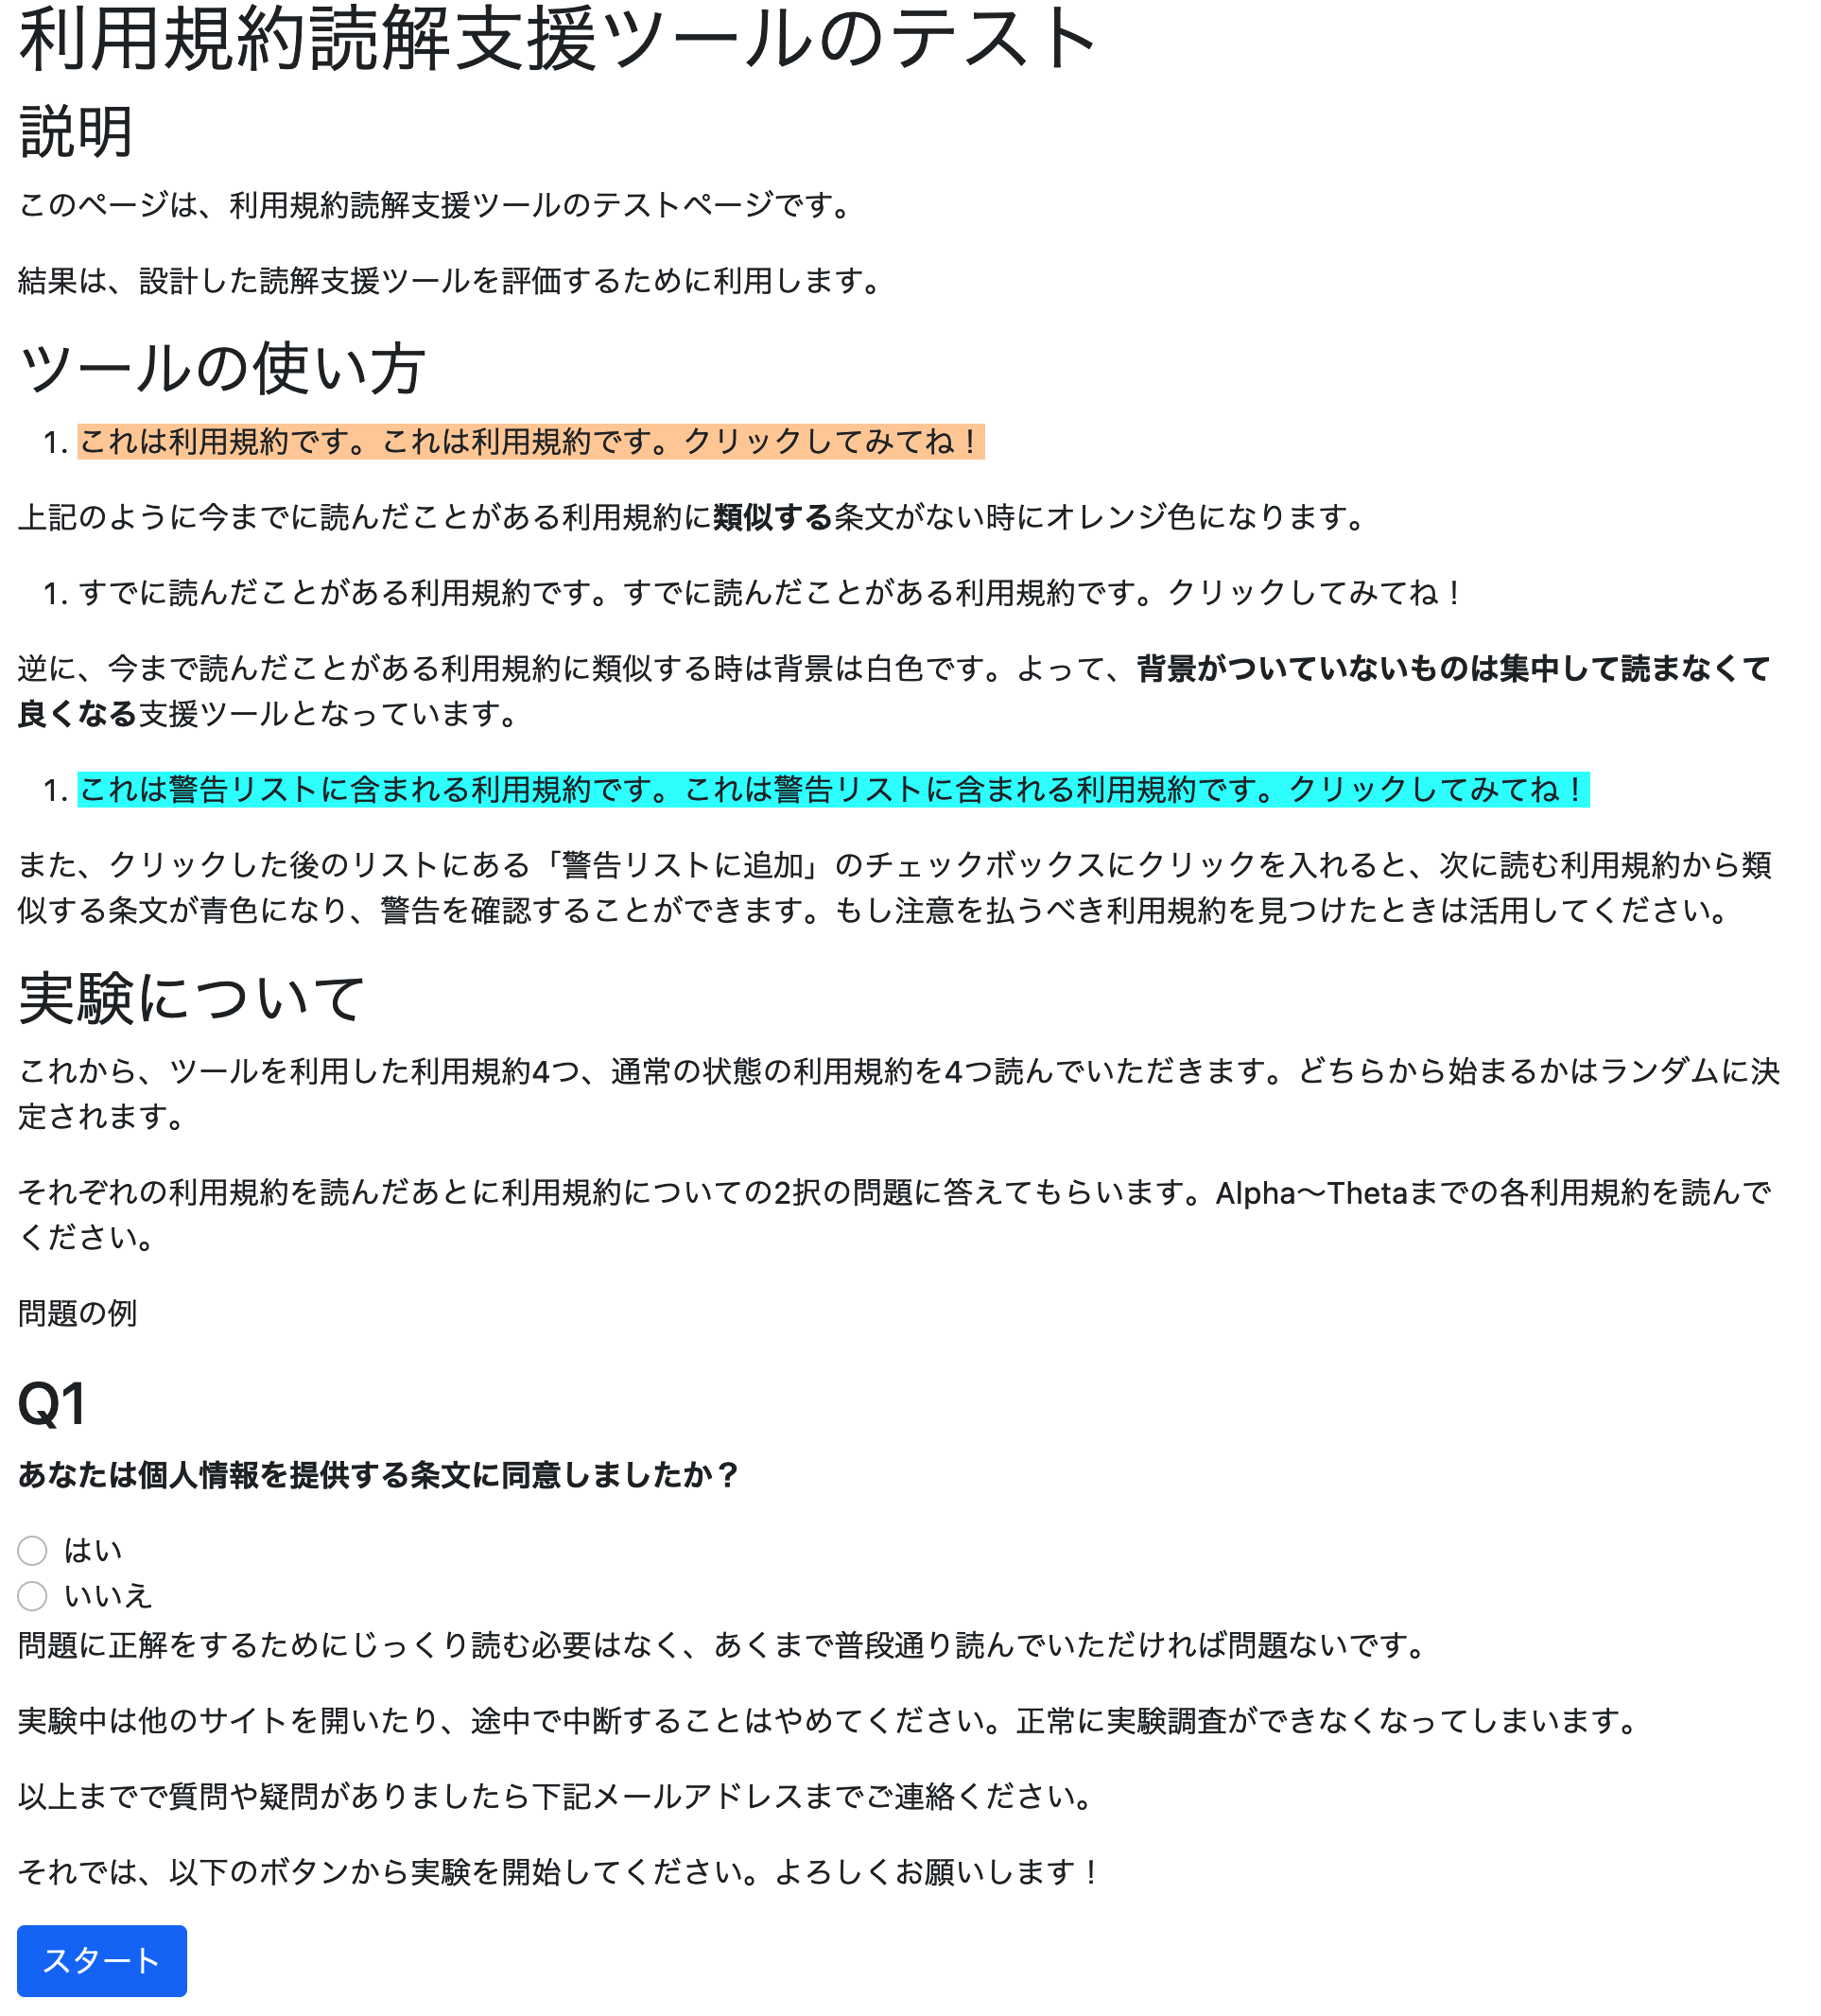
\includegraphics[width=16cm]{img/teststart1.png}
      \caption{実験概要説明ページ}
      \label{img:実験概要説明ページ}
  \end{center}
\end{figure}
被験者への説明は、「利用規約を読みやすくするためのツールのテスト」であるという表現にとどめ、本来の目的である、利用規約の読解時間短縮ということは伝えていない。これは、本来の実験の目的を最初に伝えてしまうと、被験者の読解時間の変動が起きてしまうと考えられるからである。

被験者は説明を読んだ後、利用規約を8つ読んでいく。提案システムとシステムを通さない通常の利用規約表示を比較するため、順番はランダムでかつ4つずつを読む形にした。8つの利用規約の順番もランダムであり、ランダムでどのような順序で実験が行われるかは予め被験者に通知をした。利用規約を読む時間をそれぞれ環境を作成した。また、追加実験として、8つの利用規約全てに提案システムを適用した場合の実験も行なった。
\begin{figure}[h]
  \begin{center}
      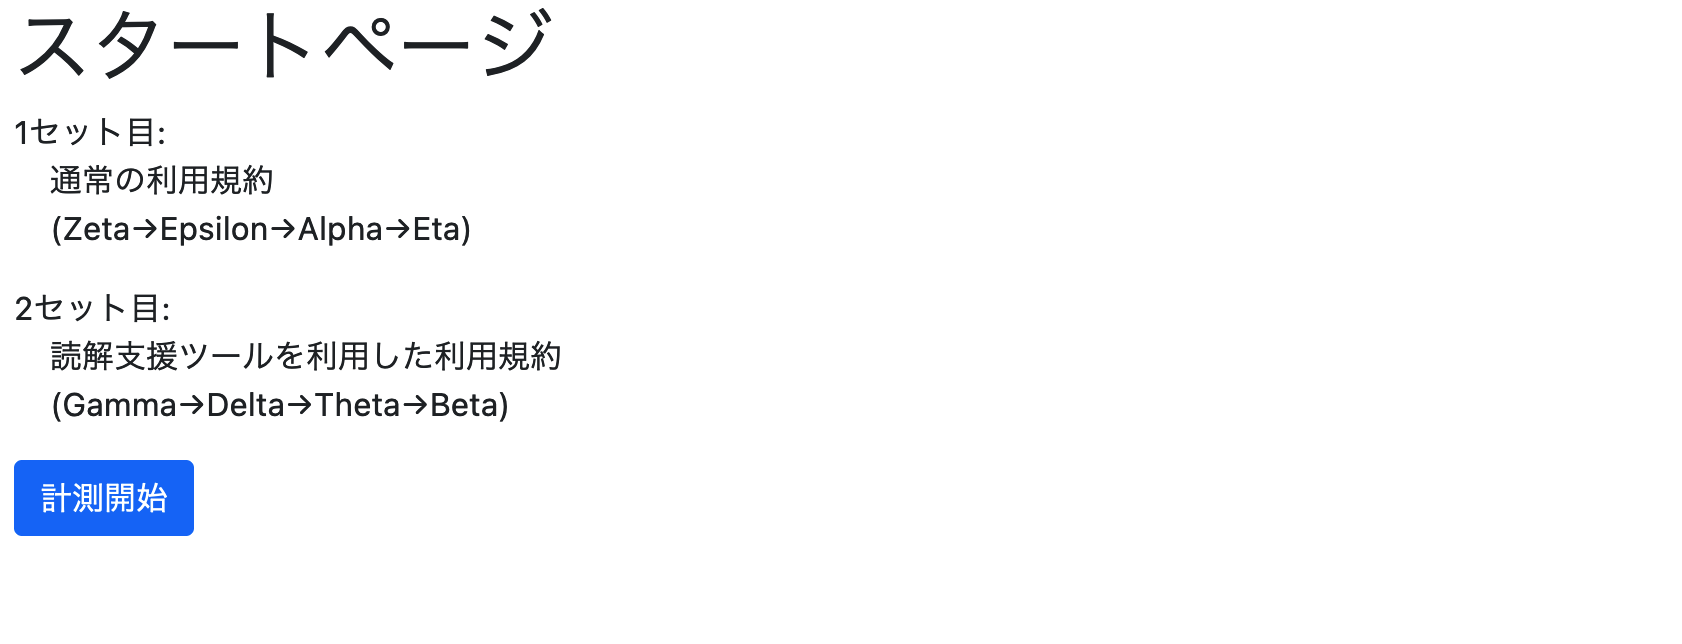
\includegraphics[width=16cm]{img/teststart2.png}
      \caption{実験順序説明ページ}
      \label{img:実験順序説明ページ}
  \end{center}
\end{figure}

そのあとは利用規約を表示し、「同意する」「同意しない」をクリックする。その後、\ref{sec:評価のためのクイズ}節で示したクイズが表示される。クイズに回答した後は次の利用規約を表示する表示が繰り返され、全ての利用規約を閲覧し終わったあとはアンケートに回答を依頼した。

\section{結果}
\ref{sec:評価用実験システムの環境}節の実験を行なった結果を示す。なお、クラウドワークス上での回答が不十分であったり、途中で実験ページから離れてしまった場合など、正常にデータを取得できなかった場合を予め除外した。通常の状態で4つ、提案システムで4つ閲覧するパターンは127件、提案システムで8つ閲覧するパターンは35件のデータを得ることができた。

\subsection{読解時間}
本提案システムは、利用規約を読んでいくごとに注目するべき部分が減ることで読解時間が減るという趣旨であるため、複数回利用規約を読む必要がある。今回の評価用実験システムは被験者の負担を考え、利用規約を4つずつ読み、読解時間を計測した。よって、通常表示の利用規約と提案システムを利用して読解した4回目を比較した。
\begin{figure}[h]
  \begin{center}
      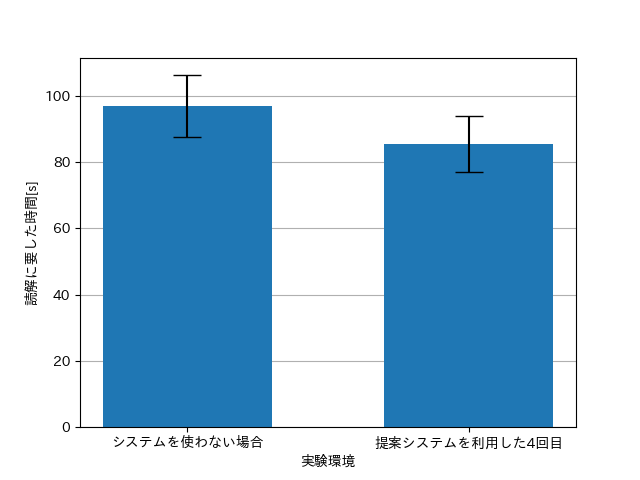
\includegraphics[width=13cm]{img/tgraph4.png}
      \caption{通常の表示の平均時間と提案システムの4回目の読解時間の比較/標準誤差}
      \label{img:通常の表示の平均時間と提案システムの4回目の読解時間の比較/標準誤差}
  \end{center}
\end{figure}
\begin{table}[h]
  \caption{通常の表示の平均時間と提案システムの4回目の読解時間}
  \label{tab:通常の表示の平均時間と提案システムの4回目の読解時間}
  \centering
  \begin{tabular}{ccc}
    \hline
    値[s]  & 通常の表示の平均時間  &  提案システムの4回目の読解時間  \\
    \hline \hline
    平均値  & 96.87  & 85.31 \\
    中央値  & 57.97   & 49.71 \\
    標準偏差  & 104.65  & 95.36 \\
    分散  &  10950.64  &  9093.15 \\
    標準誤差  &  9.29  &  8.46 \\
    \hline
  \end{tabular}
\end{table}
図\ref{img:通常の表示の平均時間と提案システムの4回目の読解時間の比較/標準誤差}、表\ref{tab:通常の表示の平均時間と提案システムの4回目の読解時間}という結果となった。対応のあるt検定で片側検定を行い、「提案システムの4回目の読解時間は通常の表示の平均時間よりも短い」という仮説を検証した結果、$p=0.03<0.05$となり、有意水準5\%でこの仮説が正しいことが示された。

また、本提案システムは利用規約を読解した量を増やしていくとさらに注目するべき部分が減っていき、さらに読むべき部分が減ると考えられる。8つ全ての利用規約を読解した場合とも比較を行う。本実験は、別の集団のため、対応がないことに留意する必要がある。
\begin{figure}[h]
  \begin{center}
      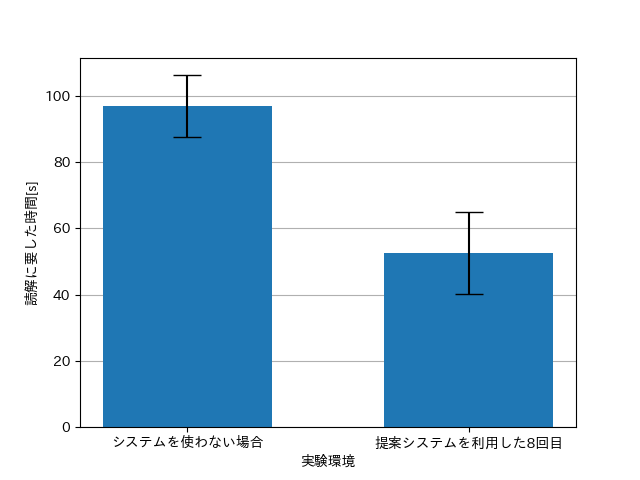
\includegraphics[width=13cm]{img/tgraph8.png}
      \caption{通常の表示の平均時間と提案システムの8回目の読解時間の比較/標準誤差}
      \label{img:通常の表示の平均時間と提案システムの8回目の読解時間の比較/標準誤差}
  \end{center}
\end{figure}
\begin{table}[h]
  \caption{提案システムの8回目の読解時間}
  \label{tab:提案システムの8回目の読解時間}
  \centering
  \begin{tabular}{ccc}
    \hline
    値[s]  & 提案システムの8回目の読解時間  \\
    \hline \hline
    平均値  & 52.50 \\
    中央値  & 28.57 \\
    標準偏差  & 72.68 \\
    分散  &  5282.13 \\
    標準誤差  & 12.28 \\
    \hline
  \end{tabular}
\end{table}
図\ref{img:通常の表示の平均時間と提案システムの8回目の読解時間の比較/標準誤差}、表\ref{tab:提案システムの8回目の読解時間}という結果になった。対応のないt検定で片側検定を行い、「提案システムの8回目を読んだ集団の読解時間は通常の表示を読んだ集団の平均読解時間よりも短い」という仮説を検証した結果、$p=0.01<0.05$となり、有意水準5\%でこの仮説が正しいことが示された。

\subsection{理解度}
提案システムを通して利用規約を読解したとき、通常の利用規約表示よりも理解度が落ちていないことを、クイズの正答率をもとに評価を行う。通常の表示を4つ、提案システムで4つ読んだ集団の正答率それぞれを比較する。
\begin{figure}[h]
  \begin{center}
      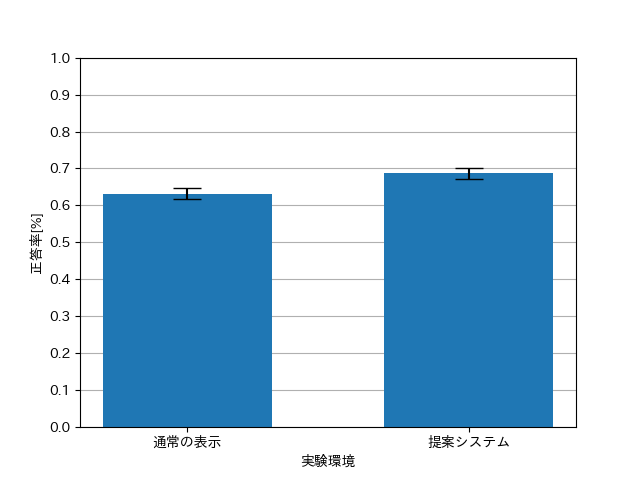
\includegraphics[width=13cm]{img/answerne4.png}
      \caption{通常の表示と提案システムの正答率の比較/標準誤差}
      \label{img:通常の表示と提案システムの正答率の比較/標準誤差}
  \end{center}
\end{figure}
\begin{table}[h]
  \caption{通常の表示と提案システムの正答率}
  \label{tab:通常の表示と提案システムの正答率}
  \centering
  \begin{tabular}{ccc}
    \hline
    正答率[\%]  & 通常の表示  &  提案システム  \\
    \hline \hline
    平均値  & 0.63  & 0.69 \\
    中央値  & 0.63   & 0.75 \\
    標準偏差  & 0.18  & 0.18 \\
    分散  &  0.03  &  0.03 \\
    標準誤差  &  0.02  &  0.02 \\
    \hline
  \end{tabular}
\end{table}
図\ref{img:通常の表示と提案システムの正答率の比較/標準誤差}、表\ref{tab:通常の表示と提案システムの正答率}という結果となった。対応のないt検定で片側検定を行い、「通常の表示よりも提案システムの正答率の方が高い」という仮説を検証した結果、$p<0.01$となり、有意水準1\%でこの仮説が正しいことが示された。また、問題ごとの正答率について個別に比較を行ったが、ほとんどの場合が提案システムの方が正答率が高かった。一部、正答率が低い場合があったが、数\%であり、検定をしても有意差は見られないため、誤差の範囲であるといえ、先述した著しく理解度が落ちていない証明ができた。

以下に、各問題についての正答率のグラフを示す。
\begin{figure}[h]
  \begin{center}
      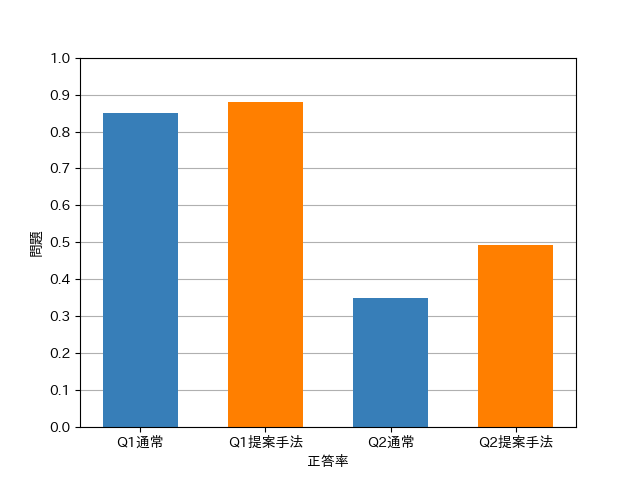
\includegraphics[width=13cm]{img/qgraphAlpha.png}
      \caption{Alpha社クイズの正答率}
      \label{img:Alpha社クイズの正答率}
  \end{center}
\end{figure}
\begin{figure}[h]
  \begin{center}
      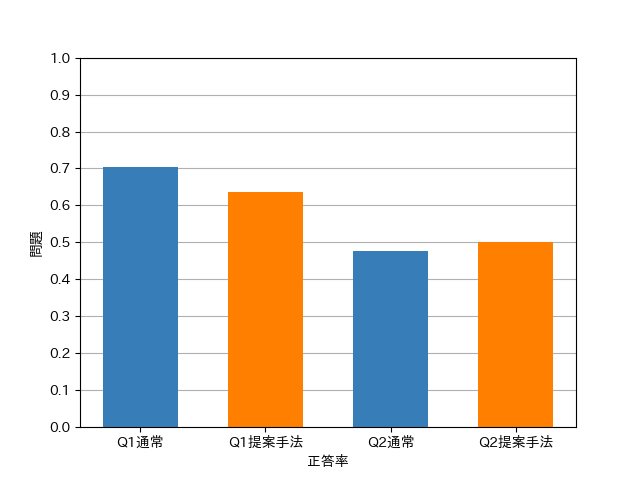
\includegraphics[width=13cm]{img/qgraphBeta.png}
      \caption{Beta社クイズの正答率}
      \label{img:Beta社クイズの正答率}
  \end{center}
\end{figure}
\begin{figure}[h]
  \begin{center}
      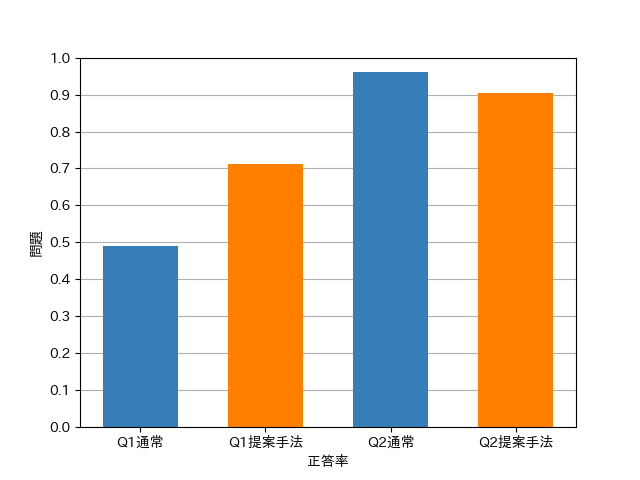
\includegraphics[width=13cm]{img/qgraphGamma.png}
      \caption{Gamma社クイズの正答率}
      \label{img:Gamma社クイズの正答率}
  \end{center}
\end{figure}
\begin{figure}[h]
  \begin{center}
      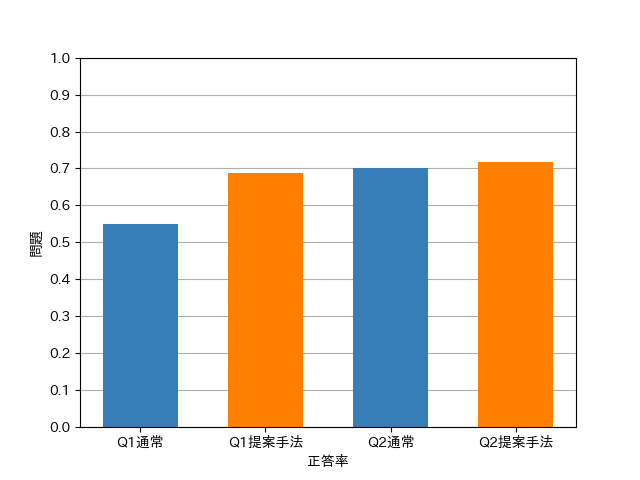
\includegraphics[width=13cm]{img/qgraphDelta.png}
      \caption{Delta社クイズの正答率}
      \label{img:Delta社クイズの正答率}
  \end{center}
\end{figure}
\begin{figure}[h]
  \begin{center}
      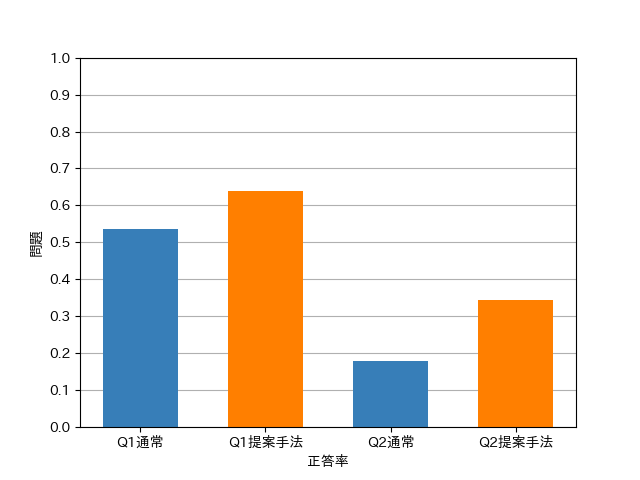
\includegraphics[width=13cm]{img/qgraphEpsilon.png}
      \caption{Epsilon社クイズの正答率}
      \label{img:Epsilon社クイズの正答率}
  \end{center}
\end{figure}
\begin{figure}[h]
  \begin{center}
      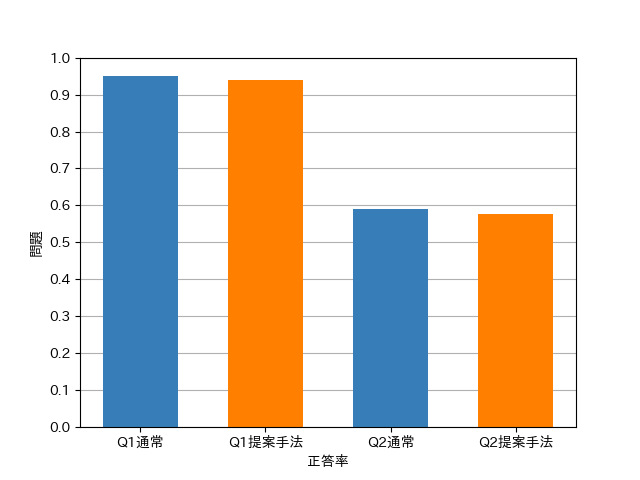
\includegraphics[width=13cm]{img/qgraphZeta.png}
      \caption{Zeta社クイズの正答率}
      \label{img:Zeta社クイズの正答率}
  \end{center}
\end{figure}
\begin{figure}[h]
  \begin{center}
      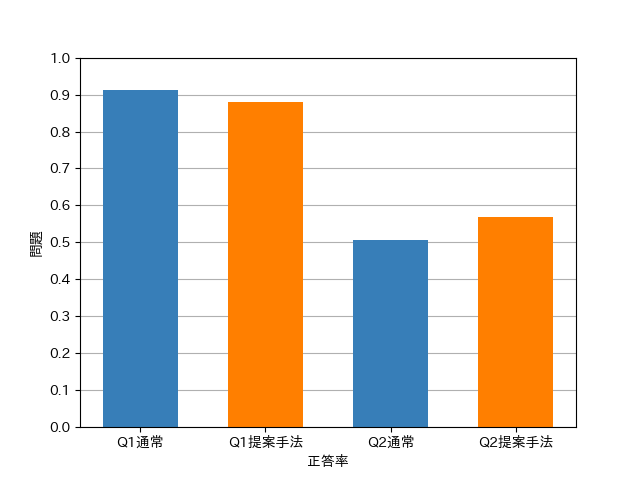
\includegraphics[width=13cm]{img/qgraphEta.png}
      \caption{Eta社クイズの正答率}
      \label{img:Eta社クイズの正答率}
  \end{center}
\end{figure}
\begin{figure}[h]
  \begin{center}
      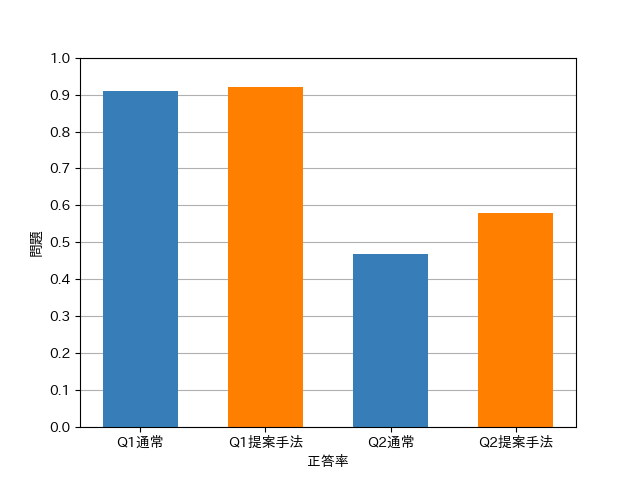
\includegraphics[width=13cm]{img/qgraphTheta.png}
      \caption{Theta社クイズの正答率}
      \label{img:Theta社クイズの正答率}
  \end{center}
\end{figure}

%%% Local Variables:
%%% mode: japanese-latex
%%% TeX-master: "./thesis"
%%% End:
